%%%%%%%%%%%%%%%%%%%%%%%%%%%%%%%%%%%%%%%%%
% Presentación Beamer - Plantilla LaTeX
% Versión 2.0 (8 de marzo de 2022)
% Plantilla original: https://www.LaTeXTemplates.com
% Autor: Vel (vel@latextemplates.com)
% Licencia: CC BY-NC-SA 4.0

% Este modelo de presentación fue 
% creado a partir del modelo de Giovanni Spadaro.
% Disponible en: https://github.com/Giovo17/presentation-template-unict-lm-data
%
% Adaptado por Lautaro Lombardi para crear una versión especial 
% para los estudiantes de Facultad de Matemática, Astronomía, Física y Computación (FAMAF - UNC).
% Disponible en: https://github.com/lautalom/beamer_FAMAF
%%%%%%%%%%%%%%%%%%%%%%%%%%%%%%%%%%%%%%%%%

%----------------------------------------------------------------------------------------
% CLASE DEL DOCUMENTO Y CONFIGURACIONES BÁSICAS
%----------------------------------------------------------------------------------------
\documentclass[
    11pt,               % Tamaño estándar de la fuente
    % t,                % Alinear verticalmente en la parte superior
    %aspectratio=169,   % Definir proporción 16:9
]{beamer}
\graphicspath{{img/}}         % Define el directorio de las imágenes

%---------------------------------------------------------------------------------------
% PAQUETES NECESARIOS
%----------------------------------------------------------------------------------------
\usepackage{
    booktabs,     % Mejora la apariencia de las líneas en tablas
    palatino,     % Define Palatino como fuente principal
    subcaption    % Soporte para subfiguras
}
\usepackage[spanish]{babel}  % Set babel to use Spanish language
\usepackage[default]{opensans}  % Define Open Sans como fuente secundaria
%----------------------------------------------------------------------------------------
% Paquetes y configuraciones para código
%----------------------------------------------------------------------------------------
% Paquetes necesarios
\usepackage[utf8]{inputenc}
\usepackage{listings}
\usepackage{xcolor}

% Colores de Visual Studio Code Light Theme
\definecolor{vscBackground}{RGB}{255,255,255}    % Fondo blanco
\definecolor{vscKeyword}{RGB}{175,0,219}         % Púrpura para palabras clave
\definecolor{vscString}{RGB}{163,21,21}          % Rojo para cadenas
\definecolor{vscComment}{RGB}{0,128,0}           % Verde para comentarios
\definecolor{vscFunction}{RGB}{121,94,38}        % Marrón para funciones
\definecolor{vscNumber}{RGB}{9,134,88}           % Verde oscuro para números
\definecolor{vscOperator}{RGB}{175,0,219}        % Púrpura para operadores
\definecolor{vscText}{RGB}{0,0,0}                % Texto negro
\definecolor{vscLineNr}{RGB}{128,128,128}        % Gris para números de línea

% Configuração geral do listings para UTF-8
\lstset{
    inputencoding=utf8,
    extendedchars=true,
    literate=%
        {á}{{\'a}}1 {é}{{\'e}}1 {í}{{\'i}}1 {ó}{{\'o}}1 {ú}{{\'u}}1
        {Á}{{\'A}}1 {É}{{\'E}}1 {Í}{{\'I}}1 {Ó}{{\'O}}1 {Ú}{{\'U}}1
        {à}{{\`a}}1 {è}{{\`e}}1 {ì}{{\`i}}1 {ò}{{\`o}}1 {ù}{{\`u}}1
        {À}{{\`A}}1 {È}{{\'E}}1 {Ì}{{\`I}}1 {Ò}{{\`O}}1 {Ù}{{\`U}}1
        {ã}{{\~a}}1 {ẽ}{{\~e}}1 {ĩ}{{\~i}}1 {õ}{{\~o}}1 {ũ}{{\~u}}1
        {Ã}{{\~A}}1 {Ẽ}{{\~E}}1 {Ĩ}{{\~I}}1 {Õ}{{\~O}}1 {Ũ}{{\~U}}1
        {â}{{\^a}}1 {ê}{{\^e}}1 {î}{{\^i}}1 {ô}{{\^o}}1 {û}{{\^u}}1
        {Â}{{\^A}}1 {Ê}{{\^E}}1 {Î}{{\^I}}1 {Ô}{{\^O}}1 {Û}{{\^U}}1
        {ç}{{\c c}}1 {Ç}{{\c C}}1
        {º}{{\textordmasculine}}1
        {ª}{{\textordfeminine}}1
}

% Configurações base comum para todas as linguagens
\lstdefinestyle{baseStyle}{
    backgroundcolor=\color{vscBackground},
    basicstyle=\ttfamily\small\color{vscText},
    breakatwhitespace=false,
    breaklines=true,
    captionpos=b,
    keepspaces=true,
    numbers=left,
    numbersep=5pt,
    showspaces=false,
    showstringspaces=false,
    showtabs=false,
    tabsize=4,
    frame=single,
    framerule=0.8pt,
    rulecolor=\color{gray!20},
    numberstyle=\tiny\color{vscLineNr},
    keywordstyle=\color{vscKeyword},
    commentstyle=\color{vscComment}\itshape,
    stringstyle=\color{vscString},
    emphstyle=\color{vscFunction},
    columns=flexible,
    basewidth={0.5em,0.45em},
    inputencoding=utf8,
    extendedchars=true
}

%----------------------------------------------------------------------------------------
% Python
%----------------------------------------------------------------------------------------
\lstdefinestyle{pythonStyle}{
    style=baseStyle,
    language=Python,
    morekeywords={self,None,True,False,import,from,as,def,class,return,yield,
                  for,while,if,else,elif,try,except,finally,with,lambda,
                  async,await,break,continue,global,nonlocal,pass,raise},
    morekeywords=[2]{print,len,range,type,int,str,float,list,dict,set,
                     tuple,max,min,sum,sorted,enumerate,zip,map,filter,
                     any,all,abs,round,pow,divmod},
    keywordstyle=[2]\color{vscFunction},
    sensitive=true
}

\lstnewenvironment{python}[1][]{\lstset{style=pythonStyle, #1}}{}
\newcommand{\pyinline}[1]{\lstinline[style=pythonStyle]!#1!}
\newcommand{\inputpython}[2][]{\lstinputlisting[style=pythonStyle,#1]{#2}}

%----------------------------------------------------------------------------------------
% C Language
%----------------------------------------------------------------------------------------
\lstdefinestyle{cStyle}{
    style=baseStyle,
    language=C,
    morekeywords={include,define,void,int,char,float,double,long,unsigned,
                  struct,union,enum,typedef,const,static,extern,register,
                  auto,volatile,sizeof,return,if,else,for,while,do,switch,
                  case,break,continue,default,goto},
    morekeywords=[2]{printf,scanf,malloc,free,calloc,realloc,fopen,fclose,
                     fprintf,fscanf,strcpy,strlen,strcat},
    keywordstyle=[2]\color{vscFunction},
    sensitive=true
}

\lstnewenvironment{clang}[1][]{\lstset{style=cStyle, #1}}{}
\newcommand{\clinline}[1]{\lstinline[style=cStyle]!#1!}
\newcommand{\inputclang}[2][]{\lstinputlisting[style=cStyle,#1]{#2}}

%----------------------------------------------------------------------------------------
% C++
%----------------------------------------------------------------------------------------
\lstdefinestyle{cppStyle}{
    style=baseStyle,
    language=C++,
    morekeywords={class,private,protected,public,template,typename,namespace,
                  using,new,delete,this,friend,virtual,override,final,explicit,
                  mutable,constexpr,nullptr,noexcept,static_cast,dynamic_cast,
                  const_cast},
    morekeywords=[2]{cout,cin,endl,vector,string,map,set,queue,stack,pair,
                     begin,end,push_back,pop_back,emplace_back,size,empty},
    keywordstyle=[2]\color{vscFunction},
    sensitive=true
}

\lstnewenvironment{cpp}[1][]{\lstset{style=cppStyle, #1}}{}
\newcommand{\cppinline}[1]{\lstinline[style=cppStyle]!#1!}
\newcommand{\inputcpp}[2][]{\lstinputlisting[style=cppStyle,#1]{#2}}

%----------------------------------------------------------------------------------------
% R Language
%----------------------------------------------------------------------------------------
\lstdefinestyle{rStyle}{
    style=baseStyle,
    language=R,
    morekeywords={if,else,repeat,while,function,for,in,next,break,TRUE,FALSE,
                  NULL,Inf,NaN,NA,NA_integer_,NA_real_,NA_complex_,NA_character_},
    morekeywords=[2]{library,require,attach,detach,source,setwd,options,
                     data.frame,read.csv,write.csv,list,matrix,array},
    keywordstyle=[2]\color{vscFunction},
    sensitive=true
}

\lstnewenvironment{rlang}[1][]{\lstset{style=rStyle, #1}}{}
\newcommand{\rlinline}[1]{\lstinline[style=rStyle]!#1!}
\newcommand{\inputrlang}[2][]{\lstinputlisting[style=rStyle,#1]{#2}}

%----------------------------------------------------------------------------------------
% Java
%----------------------------------------------------------------------------------------
\lstdefinestyle{javaStyle}{
    style=baseStyle,
    language=Java,
    morekeywords={abstract,assert,boolean,break,byte,case,catch,char,class,
                  const,continue,default,do,double,else,enum,extends,final,
                  finally,float,for,if,implements,import,instanceof,int,
                  interface,long,native,new,package,private,protected,public,
                  return,short,static,strictfp,super,switch,synchronized,this,
                  throw,throws,transient,try,void,volatile,while},
    morekeywords=[2]{String,System,out,println,printStackTrace,ArrayList,
                     HashMap,Arrays,List,Map,Set,Exception,RuntimeException},
    keywordstyle=[2]\color{vscFunction},
    sensitive=true
}

\lstnewenvironment{java}[1][]{\lstset{style=javaStyle, #1}}{}
\newcommand{\javainline}[1]{\lstinline[style=javaStyle]!#1!}
\newcommand{\inputjava}[2][]{\lstinputlisting[style=javaStyle,#1]{#2}}       % Importa configuraciones para resaltar código

%---------------------------------------------------------------------------------------
% CONFIGURACIÓN DEL TEMA
%----------------------------------------------------------------------------------------
% Tema Base
\usetheme{Boadilla}                          % Define el tema principal
\useinnertheme{circles}                      % Tema interno con círculos
\useoutertheme{miniframes}                   % Tema externo con miniframes
\setbeamertemplate{navigation symbols}{}     % Elimina símbolos de navegación

% Colores Personalizados
\definecolor{primaryColor}{RGB}{11, 139, 171} % Color primario - cian Famaf oficial
\definecolor{secondaryColor}{RGB}{0, 104, 128}    % Color secundario - azul verdoso

% Configuraciones de Colores
\setbeamercolor{structure}{fg=primaryColor}
\setbeamercolor{palette primary}{bg=primaryColor, fg=white}
\setbeamercolor{palette secondary}{bg=secondaryColor, fg=white}
\setbeamercolor{title}{bg=primaryColor, fg=white}

% Colores del Encabezado y Pie de Página
\setbeamercolor{headline}{bg=secondaryColor, fg=white}
\setbeamercolor{section in head/foot}{bg=primaryColor, fg=white}
\setbeamercolor{subsection in head/foot}{bg=secondaryColor, fg=white}
\setbeamercolor{author in head/foot}{bg=primaryColor, fg=white}
\setbeamercolor{title in head/foot}{bg=secondaryColor, fg=white}
\setbeamercolor{date in head/foot}{bg=primaryColor, fg=white}
\setbeamercolor{page number in head/foot}{bg=primaryColor, fg=white}

%----------------------------------------------------------------------------------------
% BIBLIOGRAFÍA
%----------------------------------------------------------------------------------------
\bibliographystyle{plain}
%----------------------------------------------------------------------------------------
% INFORMACIÓN DE LA PRESENTACIÓN
%----------------------------------------------------------------------------------------
\title[Swaptions en LMM]{Valoración de Swaptions en el Modelo de Mercado Libor}          % [Versión corta]{Versión completa}
\author[Lautaro Lombardi]{Lautaro Lombardi}        % [Versión corta]{Nombre completo}
\institute[FAMAF]{Facultad de Matemática, Astronomía, Física y Computación \\ (FAMAF - UNC) }
\date[2025]{Mayo 2025}                                % [Versión corta]{Fecha completa}   

%----------------------------------------------------------------------------------------
% INICIO DEL DOCUMENTO
%----------------------------------------------------------------------------------------
\begin{document}
% Diapositiva de título con logo
\newtheorem{defin}{Definición}[section]
\newtheorem{thm}{Teorema}[section]
\newtheorem{prop}{Proposicion}[section]
\newtheorem{obs}{Observación}[section]
\newtheorem{notat}{Notación}[section]

\begin{frame}
    \begin{figure}
        
\includegraphics[width=0.50\linewidth]{img/famaf.png} % Adjusted width
    \end{figure}
    \titlepage
\end{frame}

% Sumario
\begin{frame}
    \frametitle{Estructura de la presentación}
    \tableofcontents
\end{frame}

% Inclusión de las secciones
\section{Tasas de interés y derivados}

\begin{frame}
% center the title
    \begin{center}
        \textbf{\huge Tasas de interés y derivados}
    \end{center}
\end{frame}
%----------------------------------------------------------------------------------------

\begin{frame}
    \frametitle{Tasa de interés simple}
    Si A le presta un monto \$1 en tiempo $T_1$ a B y B le paga un monto \$1 en tiempo $T_2$ más cierto interés K entre $T_1$ y $T_2$. 
    \begin{figure}[h]
       \centering
       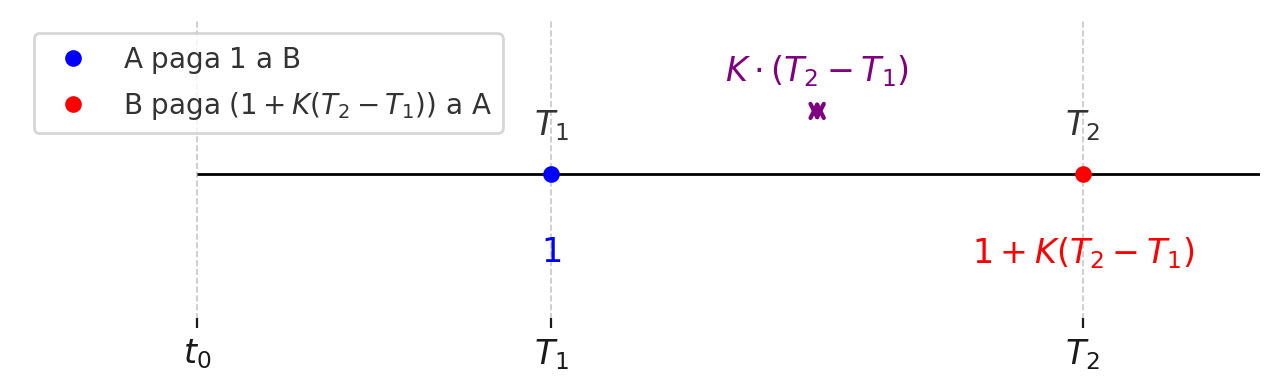
\includegraphics[width=\textwidth]{img/cap1/accrual_simple.png}
       \caption{Tasa simple}
       \label{accrual_simple}
   \end{figure}
\end{frame}

%----------------------------------------------------------------------------------------

\begin{frame}
    \frametitle{Sistemas de Capitalización}
    Un interés de \$100 a una tasa de 10\% anual con capitalización semestral durante 3 años resulta en
    \begin{itemize}
        \item \textbf{Capitalización Simple:} $100 \times (1+\frac{0.1}{2} \times 6) = 130$.
        \item \textbf{Capitalización Compuesta Discreta:} $100 \times (1+0.1/2)^{2 \times 3} = 133.1$.  
        \item \textbf{Capitalización Compuesta Continua:} $100 \times e^{0.1 \times 3} = 134.98$. 
    \end{itemize}

\end{frame}

%----------------------------------------------------------------------------------------

\begin{frame}
    \frametitle{Bonos cupon cero}
    Componentes:
    \begin{itemize}
        \item \textbf{Valor nominal (N):} Monto a pagar al vencimiento.
        \item \textbf{Tasa de interés (r):} Tasa \textit{cero} anual.
        \item \textbf{Tiempo hasta el vencimiento (T):} Tiempo en años hasta el vencimiento.
        \item \textbf{Precio (P):} Precio actual del bono.
    \end{itemize}
    % side by side equations
    \begin{columns}
        \column{0.4\textwidth}
            \begin{equation*}
                P = \frac{N}{(1+r)^T}
            \end{equation*}
        \column{0.4\textwidth}
            \begin{equation*}
                P = N \cdot e^{-rT}
            \end{equation*}
    \end{columns}
\end{frame}

%----------------------------------------------------------------------------------------

\begin{frame}
    \frametitle{Valoración de un bono con cupones}
    Consideremos un bono de principal \$100, madurez en 2 años y tasa cupón 5\% semianual.\\
    Supongamos que las tasas cero a 6 meses, 1 año, 1.5 años y 2 años son 4\%, 4.5\%, 5\% y 5.5\% respectivamente.\\
    \begin{itemize}
        \item \textbf{Flujos de caja:} \$2.5, \$2.5, \$2.5, \$102.5
        \item \textbf{Tasas cero:} 4\%, 4.5\%, 5\%, 5.5\%
        \item \textbf{Precios:} $\$2.5 \cdot e^{-0.04 \cdot 0.5} + \$2.5 \cdot e^{-0.045 \cdot 1} + \$2.5 \cdot e^{-0.05 \cdot 1.5} + \$102.5 \cdot e^{-0.055 \cdot 2}$
        \item \textbf{Precio total:} 98.98
    \end{itemize}
\end{frame}
%----------------------------------------------------------------------------------------

\begin{frame}
    \frametitle{Modelo de tasas de interés}
    \begin{defin}[cuenta de moneda]
        Activo que capitaliza intereses a una tasa de interés r libre de riesgo entre [0, T].\\
        \begin{equation*}
            B(0) = 1 
        \end{equation*}
        \begin{equation*}
            dB(t) = rB(t)dt
        \end{equation*}
        \begin{equation*}
            B(t) = B(0)e^{rt}
        \end{equation*}
        \begin{equation*}
            B(t) = B(0)e^{\int_0^t r(s)ds}
        \end{equation*}
    \end{defin}
\end{frame}

%----------------------------------------------------------------------------------------

\begin{frame}
    \frametitle{Valor inicial de un flujo de caja}
    \begin{defin}[Valor inicial]
        El valor en t=0 de \$1 en t=T es A tal que:
        \begin{equation*}
            A \times B(T) = 1
        \end{equation*}
        \begin{equation*}
            A = \frac{1}{B(T)} = e^{-rT}
        \end{equation*}
        \begin{equation*}
            A = e^{-\int_0^T r(s)ds}
        \end{equation*}
    \end{defin}
\end{frame}
%----------------------------------------------------------------------------------------

\begin{frame}
    \frametitle{Valor presente}
    \begin{defin}[Factor de descuento]
        En $t<T$ el valor presente de \$1 en T es:
        \begin{equation*}
            \frac{1}{B(T)} \times B(t) = \frac{B(t)}{B(T)}
        \end{equation*}
        \begin{equation*}
           D_B(t,T) = \frac{B(t)}{B(T)}
        \end{equation*}
    \end{defin}
\end{frame}

%----------------------------------------------------------------------------------------

\begin{frame}
    \frametitle{Bono cupón cero}
    \begin{defin}[Bono cupón cero]
        Un bono cupón cero P(t,T) es el valor observado en t de un contrato que paga \$1 en T.
        \begin{equation*}
            P(T, T) = 1
        \end{equation*}
        \begin{align*}
            P(t, T) &= D_B(t,T) \\
            &= \frac{B(t)}{B(T)} \\
            \text{si r es estocástica}\\
            &\stackrel{?}{=} D_B(t,T) \\
              &= \mathbb{E}^{\text{???}}\left[\frac{B(t)}{B(T)}\right] \\
        \end{align*}
    \end{defin}
\end{frame}

%----------------------------------------------------------------------------------------

\begin{frame}
    \frametitle{Tasas spot}
    \begin{defin}[Tasa spot simple]
        Es la tasa de interés L vigente entre [S,T] tal que:
        \begin{equation*}
            P(S,T) \times (1+L(S,T) (T-S)) = 1
        \end{equation*}
    \end{defin}
    \begin{defin}[Tasa spot compuesta]
        Es la tasa de interés R vigente entre [S,T] tal que:
        \begin{equation*}
            P(S,T) \times (1+R(S,T))^{(T-S)} = 1
        \end{equation*}
    \end{defin}
\end{frame}
%----------------------------------------------------------------------------------------

\begin{frame}
    \frametitle{Tasas forward}
    Son tasas implícitas por las tasas spot.
    \begin{itemize}
        \item Sean las tasas spot a 1 y 2 años conocidas e iguales a 3 y 4\% respectivamente.
        \item entonces la tasa forward f entre el año 1 y 2 es tal que
        \[e^{0.03} \cdot e^{f(0,1,2)} = e^{0.04 \cdot 2} \therefore f(0,1,2)=0.05 \]
    \end{itemize}
        \begin{figure}[h]
        \centering
        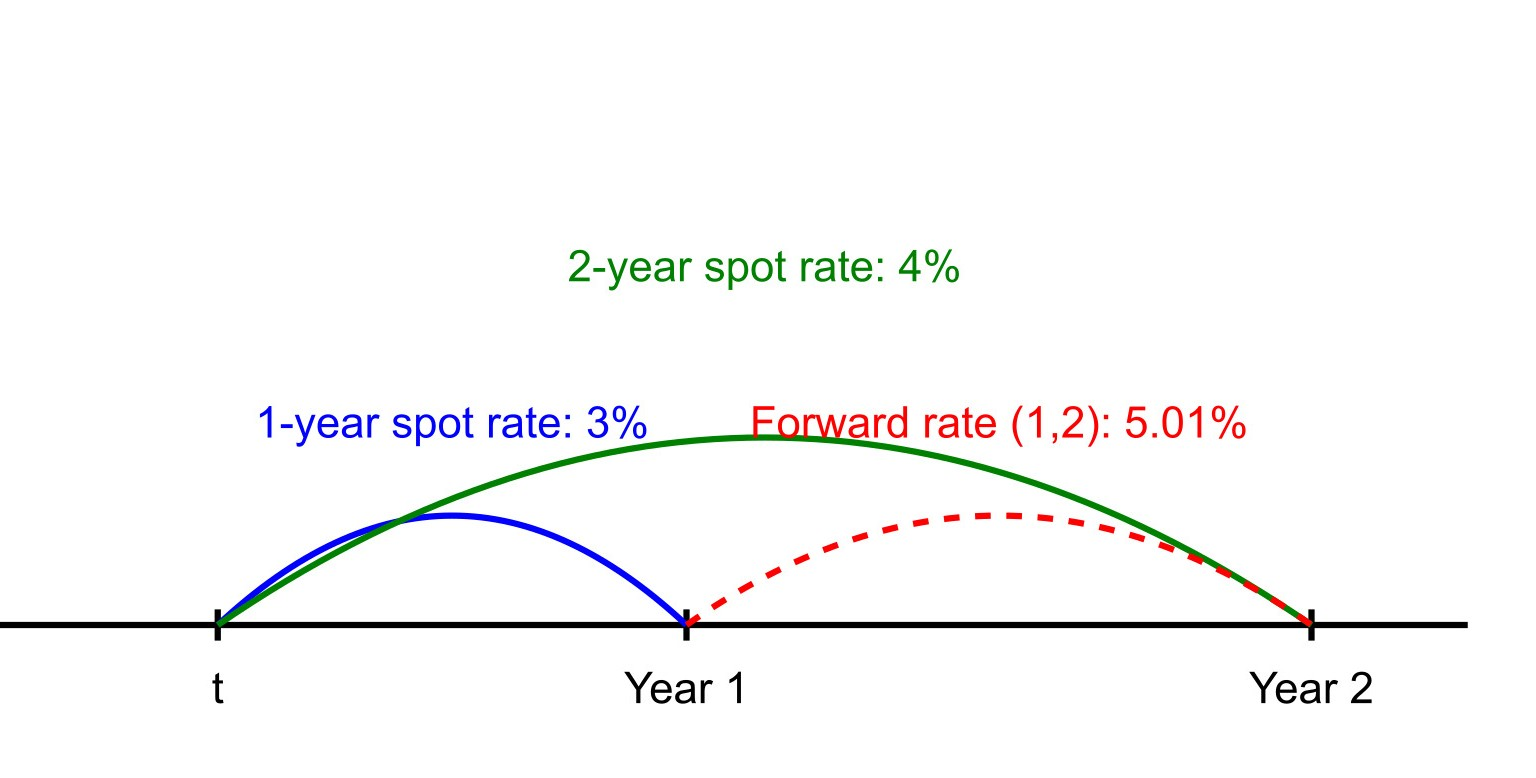
\includegraphics[width=0.8\textwidth]{img/cap1/forward-rates.jpg}
        \caption{Tasas forward}
        \label{forward_rates}
    \end{figure}
\end{frame}

%----------------------------------------------------------------------------------------

\begin{frame}
    \frametitle{Bonos y tasas forward}
    Para capturar un bono que se emitirá en el futuro deberíamos
    \begin{itemize}
        \item Comprar un (1) BCC con madurez $T_2$ y vender alguna cantidad BCC con madurez $T_1$.
        \item El costo de la estrategia es:
        \begin{equation*}
            -1 \cdot P(T_0,T_2) + \frac{P(T_0,T_2)}{P(T_0,T_1)} \cdot P(T_0,T_1) = 0
        \end{equation*}
    \end{itemize}
    \begin{defin}[Bono forward]
        Un bono forward es un contrato que paga \$1 en el tiempo $T_2$ y cuyo precio es
        \begin{equation*}
            P(T_0, T_1, T_2) = \frac{P(T_0,T_2)}{P(T_0,T_1)}
        \end{equation*}
    \end{defin}
\end{frame}

%----------------------------------------------------------------------------------------

\begin{frame}
    \frametitle{Tasas forward}
    \begin{defin}[Tasa forward simple]
        Es la tasa de interés L vigente entre [T,T+$\tau$] tal que:
        \begin{equation*}
            L(t, T, T+\tau) = \frac{1}{\tau} \left( \frac{1}{P(t, T, T+\tau)} - 1\right)
        \end{equation*}
    \end{defin}
    \begin{defin}[Tasa forward continua]
        Es la tasa de interés R vigente entre [T,T+$\tau$] tal que:
        \begin{equation*}
            R(t, T, T+\tau) = \frac{1}{\tau} \cdot \ln\left(\frac{1}{P(t, T, T+\tau)}\right)
        \end{equation*}
    \end{defin}
\end{frame}
%----------------------------------------------------------------------------------------

\begin{frame}
    \frametitle{Tasas forward}
    \begin{notat}
        Denotamos $L_j(t)$ a la tasa forward $L(t, T_j, T_{j+1})$.
    \end{notat}

\end{frame}

%----------------------------------------------------------------------------------------
\begin{frame}
    \begin{center}
        \textbf{\huge Derivados}
    \end{center}
\end{frame}

%----------------------------------------------------------------------------------------

\begin{frame}
    \frametitle{Derivados}
    \begin{defin}[Derivado]
        Un derivado es un contrato cuyo pago es una función de un activo subyacente S en algún momento T.
        \[V(T) = f(S(T))\]
    \end{defin}
\end{frame}
%----------------------------------------------------------------------------------------

\begin{frame}
    \frametitle{Opciones}
    \begin{defin}[Opcion]
        Una opción tiene un desembolso (payoff) que depende del subyacente y un umbral.\\
        \begin{itemize}
            \item Base o strike: umbral para ejercicio.
            \item Fecha de ejercicio: europeas < bermudas < americanas.
            \item Prima: Precio de la opción.
        \end{itemize}
    \end{defin}
\end{frame}

%----------------------------------------------------------------------------------------

\begin{frame}
    \frametitle{Derivados: C50}
    \begin{figure}[h]
       \centering
       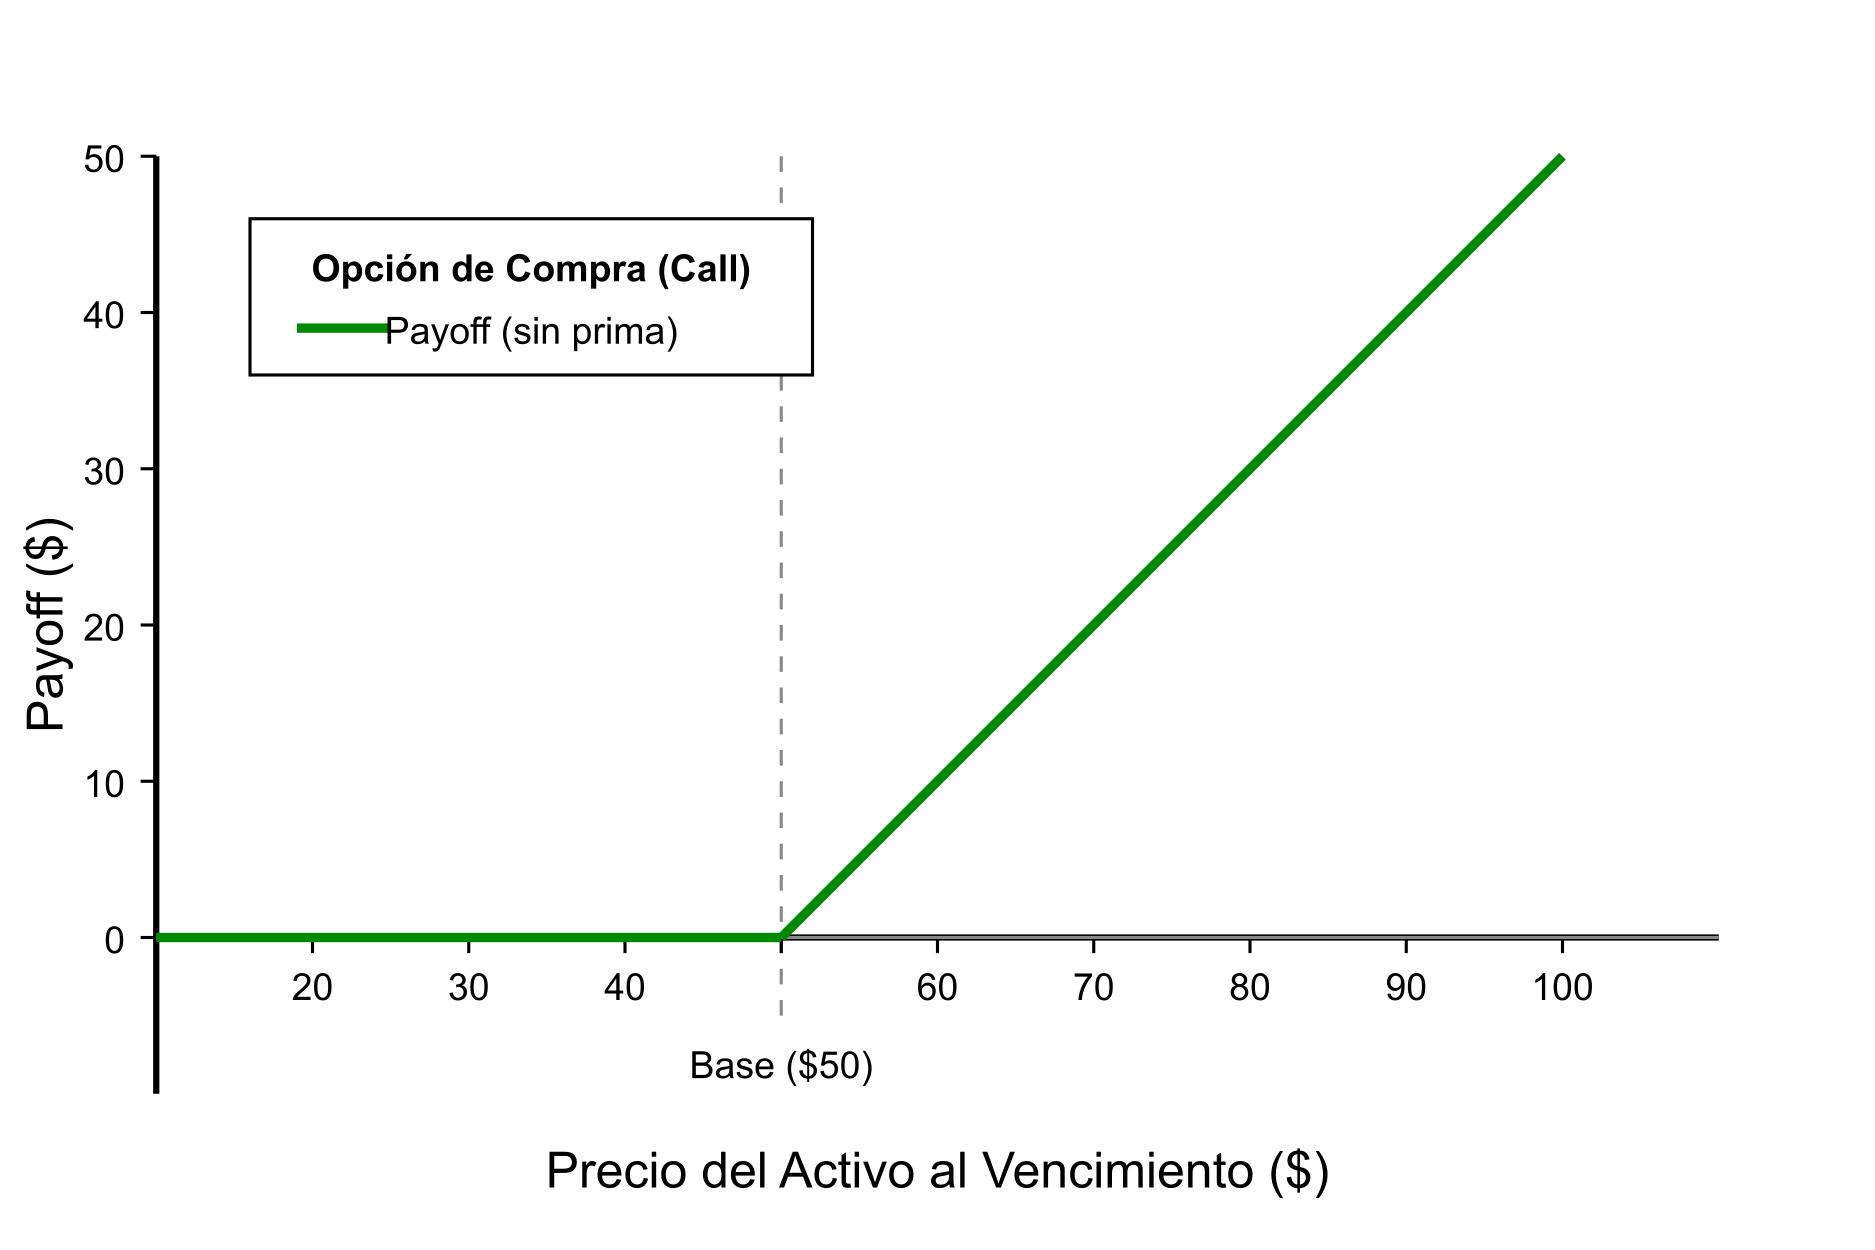
\includegraphics[width=0.8\textwidth]{img/cap1/call50.jpg}
       \caption{Call base 50}
       \label{Call50}
    \end{figure}
\end{frame}

%----------------------------------------------------------------------------------------

\begin{frame}
    \frametitle{FRA}
    \begin{defin}[FRA]
        Un FRA es un contrato que paga la diferencia entre la tasa fija K y otra variable L entre dos fechas $[T_1,T_2]$.
        \begin{itemize}
            \item t=0: fecha de inicio del contrato.
            \item $T_1$: fecha en la que conozco la tasa $L(T_1,T_2)$.
            \item $T_2$: fecha de pago.
        \end{itemize}
        \begin{align*}
            \text{Payoff}_{\text{Short}} &= N (K - L(T_1,T_2)) \cdot (T_2 - T_1), \\
            \text{Payoff}_{\text{Long}} &= N (L(T_1,T_2) - K) \cdot (T_2 - T_1). \\
            \text{K}_\text{FRA} &= L(0, 1, 2) = L_1(0)
        \end{align*}
    \end{defin}
\end{frame}

%----------------------------------------------------------------------------------------

\begin{frame}
    \frametitle{Swap}
    \begin{defin}[Swap]
        \begin{itemize}
            \item Nominal N, Tasa fija K, Tasa variable L
            \item Tiempos de Observación de L: $T_0, T_1, \ldots, T_{n-1}$
            \item Tiempos de pago; $T_1, T_2, \ldots, T_{n}$
            \item Tenor: $T_i - T_{i-1}= \tau_i$
            \item Pago long en cada $T_i$: $N\cdot \tau_i \cdot K$
            \item Pago short en cada $T_i$: $N\cdot \tau_i \cdot L(T_{i-1}, T_i)$
        \end{itemize}
        \begin{align*}
            \text{Payoff}_{\text{Long}} &= N \sum_{i=1}^n \tau_i (L(T_{i-1}, T_i) - K). \\
            \text{K}_\text{Swap} &= \frac{\sum_{j=1}^n P(t, T_{j+1}) (T_{j+1} - T_j) L_j(t)}{\sum_{j=1}^n P(t, T_{j+1}) (T_{j+1} - T_j)}
        \end{align*}
    \end{defin}
\end{frame}

%----------------------------------------------------------------------------------------

\begin{frame}
    \frametitle{Swap: Ejemplo}
    \begin{itemize}
        \item Nominal \$1000, tasa fija 5\%, tasa variable L.
        \item Tiempos de observación de L: 1, 2, 3, 4 años.
        \item Tiempos de pago: 2, 3, 4, 5 años.
        \item Tenor: 1 año.
        \item Pago long en cada $T_i$: \$50
        \item Pago short en cada $T_i$: $L(T_{i-1}, T_i)$
    \end{itemize}
    \begin{align*}
        \text{Payoff}_{\text{Short}} &= \$1000 \cdot \sum_{i=1}^4 (1) (5\% - L(T_{i-1}, T_i)) \\
        \text{Payoff}_{\text{Long}} &= \$1000 \cdot \sum_{i=1}^4 (1) (L(T_{i-1}, T_i) - 5\%)
    \end{align*}
\end{frame}

%----------------------------------------------------------------------------------------

\begin{frame}
    \frametitle{Cap}
    \begin{defin}[Cap]
        Similar al swap, pero el pago es el máximo entre la tasa variable y la tasa fija.
        \begin{align*}
            \text{Payoff}_{\text{Short}} &= N \sum_{i=1}^n \tau_i (K - L(T_{i-1}, T_i))^+ \\
            \text{Payoff}_{\text{Long}} &= N \sum_{i=1}^n \tau_i (L(T_{i-1}, T_i) - K)^+
        \end{align*}
        Compuesto por \textit{caplets}.
    \end{defin}
\end{frame}

%----------------------------------------------------------------------------------------

\begin{frame}
    \frametitle{Floor}
    \begin{defin}[Floor]
        Similar al swap, pero el pago es el mínimo entre la tasa variable y la tasa fija.
        \begin{align*}
            \text{Payoff}_{\text{Short}} &= N \sum_{i=1}^n \tau_i (K - L(T_{i-1}, T_i))^- \\
            \text{Payoff}_{\text{Long}} &= N \sum_{i=1}^n \tau_i (L(T_{i-1}, T_i) - K)^-
        \end{align*}
        Compuesto por \textit{floorlets}.
    \end{defin}
\end{frame}

%----------------------------------------------------------------------------------------

\begin{frame}
    \frametitle{Swaption}
    \begin{defin}[Swaption]
        Un swaption es un contrato que otorga el derecho, pero no la obligación, de entrar en un swap.
        \begin{equation*}
        \text{Payoff}_{T_0} = \max\left(0, N \sum_{i=1}^n \tau_i (L(T_{i-1}, T_i) - K)\right)
        \end{equation*}
    \end{defin}
\end{frame}


\section{Movimiento Browniano}

%----------------------------------------------------------------------------------------

\begin{frame}
%center the title
    \begin{center}
        \textbf{\huge Movimiento Browniano}
    \end{center}
\end{frame}

%----------------------------------------------------------------------------------------

\begin{frame}
    \frametitle{Procesos Estocásticos}
    \begin{itemize}
        \item Variables que cambian de valor en el tiempo de forma incierta.
        \item Clasificación: tiempo discreto o continuo, variable continua o discreta.
        \item Definición formal: un proceso estocástico es una colección de variables aleatorias indexadas por el tiempo.
        \[X: \Omega \times I \rightarrow \mathbb{R}\]
    \end{itemize}
\end{frame}

%----------------------------------------------------------------------------------------

\begin{frame}
    \frametitle{Definición del Proceso \( S_t(\omega_1 \omega_2 \omega_3) \)}
    
    \[
    S_0(\omega_1 \omega_2 \omega_3) = 4 \quad \text{para todo } \omega_1 \omega_2 \omega_3 \in \Omega_3,
    \]
    
    \[
    S_1(\omega_1 \omega_2 \omega_3) =
    \begin{cases}
        8 & \text{si } \omega_1 = C, \\
        2 & \text{si } \omega_1 = N,
    \end{cases}
    \]
    
    \[
    S_2(\omega_1 \omega_2 \omega_3) =
    \begin{cases}
        16 & \text{si } \omega_1 = \omega_2 = C, \\
        4 & \text{si } \omega_1 \ne \omega_2, \\
        1 & \text{si } \omega_1 = \omega_2 = N,
    \end{cases}
    \]
    
    \[
    S_3(\omega_1 \omega_2 \omega_3) =
    \begin{cases}
        32 & \text{si } \omega_1 = \omega_2 = \omega_3 = C, \\
        8 & \text{si hay dos caras y una cruz}, \\
        2 & \text{si hay una cara y dos cruces}, \\
        0.5 & \text{si } \omega_1 = \omega_2 = \omega_3 = N.
    \end{cases}
    \]

\end{frame}

%----------------------------------------------------------------------------------------

\begin{frame}
    \frametitle{Evolución de $S_t$}
    \begin{figure}
        \centering
        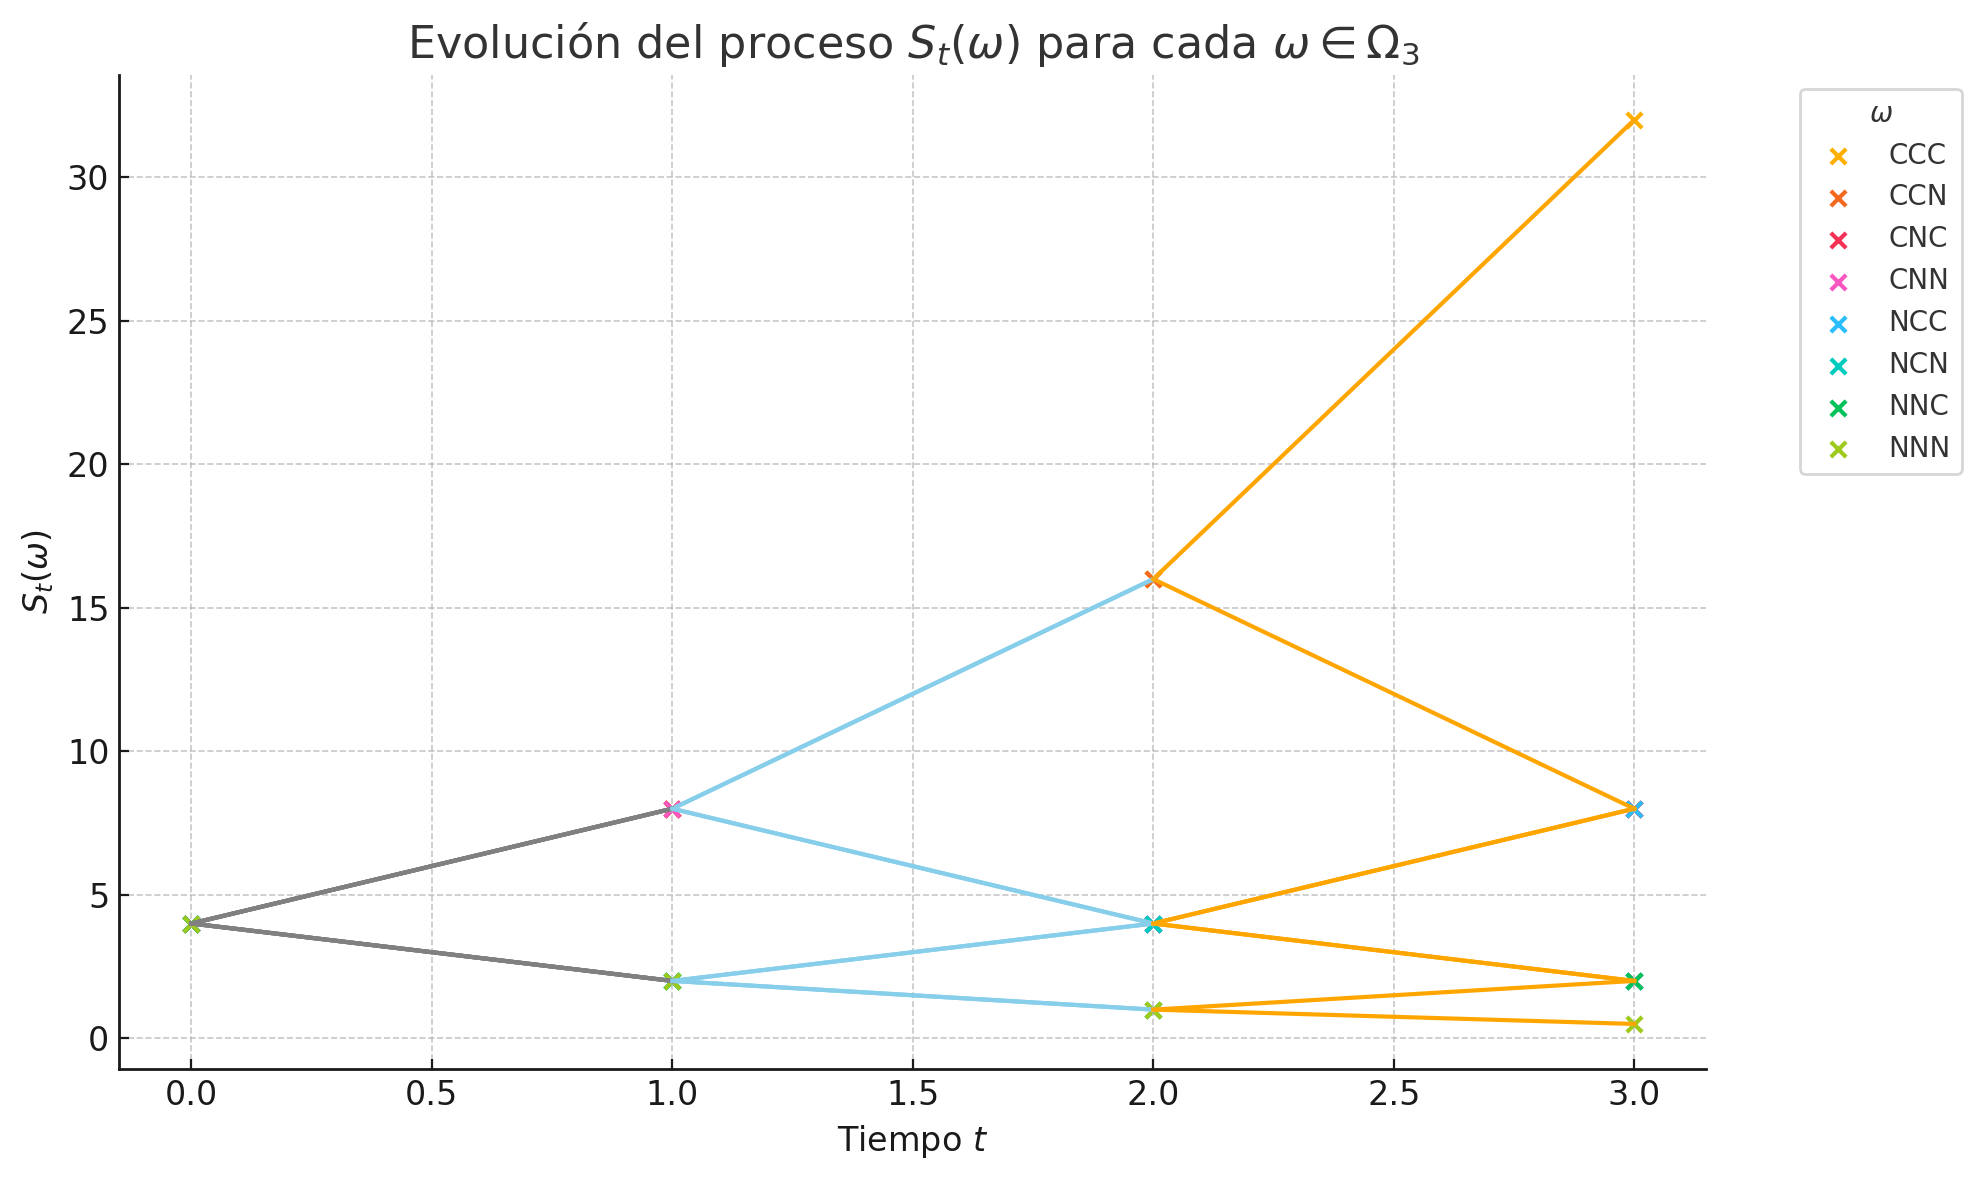
\includegraphics[width=0.8\textwidth]{img/cap2/S_t.jpg}
        \caption{Evolución del proceso $S_t$ en el tiempo.}
        \label{fig:evolucion}
    \end{figure}
\end{frame}

%----------------------------------------------------------------------------------------
\begin{frame}
    \frametitle{Movimiento Browniano}
    \begin{itemize}
        \item Proceso continuo que comienza en 0: \(W(0) = 0\).
        \item Incrementos independientes y distribuidos normalmente.
        \item Propiedades:
        \begin{itemize}
            \item \(\mathbb{E}[W(t)] = 0\).
            \item \(\text{Var}[W(t)] = t\).
        \end{itemize}
    \end{itemize}
\end{frame}

%----------------------------------------------------------------------------------------

\begin{frame}
    \frametitle{Valor Esperado Condicional}
    \begin{itemize}
        \item Definición: \(\mathbb{E}[X|\mathcal{G}]\) satisface medibilidad y promedio parcial.
        \item Propiedades:
        \begin{itemize}
            \item Linealidad.
            \item Condicionamiento iterado.
            \item Desigualdad de Jensen.
        \end{itemize}
    \end{itemize}
\end{frame}

%----------------------------------------------------------------------------------------

\begin{frame}
    \frametitle{Martingalas}
    \begin{itemize}
        \item Proceso estocástico sin deriva.
        \item Propiedad clave: \(\mathbb{E}[M(t)|\mathcal{F}(s)] = M(s)\).
        \item Ejemplo: Movimiento Browniano es una martingala.
    \end{itemize}
\end{frame}

%----------------------------------------------------------------------------------------

\begin{frame}
    \frametitle{Proceso de Itô}
    \begin{itemize}
        \item Modelo para capturar la naturaleza estocástica de los precios de activos financieros.
        \item Representación general:
        \[dX = \mu(X, t) \, dt + \sigma(X, t) \, dW\]
        \item \(\mu\): tasa de deriva. \(\sigma\): volatilidad.
    \end{itemize}
\end{frame}

%----------------------------------------------------------------------------------------

\begin{frame}
    \frametitle{Lema de Itô}
    \begin{itemize}
        \item Relaciona una función \(G(X, t)\) con el proceso de Itô subyacente.
        \item Fórmula:
        \[dG = \frac{\partial G}{\partial t} \, dt + \frac{\partial G}{\partial X} \, dX + \frac{1}{2} \frac{\partial^2 G}{\partial X^2} \, (\sigma^2 \, dt)\]
        \item Aplicación: valuación de derivados financieros.
    \end{itemize}
\end{frame}
% Diapositiva final
\begin{frame}
    \begin{center}
        {\Huge ¡Fin de la presentación!}
    \end{center}
\end{frame}

\end{document}

